%%%%%%%%%%%%%%%%%%%%%%%%%%%%%%%%%%%%%%%%%%%%%%%%%%%%%%
\documentclass[11pt]{article}
%%%%%%%%%%%%%%%%%%%%%%%%%%%%%%%%%%%%%%%%%%%%%%%%%%%%%%

\usepackage{amsmath}
\usepackage{amsthm}
\usepackage{amssymb}
\usepackage{latexsym}
\usepackage{graphicx}
\usepackage{color}
\usepackage{verbatim}
\usepackage{float}
\usepackage{multicol}
\usepackage{xcolor}
\usepackage{listings}
\usepackage{tikz}
\usetikzlibrary{arrows.meta, positioning, calc}
\usetikzlibrary{decorations.pathmorphing}
\usepackage{tcolorbox}
\tcbuselibrary{breakable}
\usepackage{cancel}


\newtcolorbox{solutionbox}{
  breakable,
  colback=blue!5!white,
  colframe=blue!50!black,
  title=Solution,
  sharp corners,
  boxrule=0.8pt
}

\newtcolorbox{hintbox}{
  breakable,
  colback=gray!10!white,
  colframe=gray!50!black,
  title=Hint,
  sharp corners,
  boxrule=0.5pt
}

% Unnumbered theorem
\newtheorem*{thm*}{Theorem}

\lstdefinelanguage{R}{
      keywords={if,else,while,for,in,next,break,function,TRUE,FALSE,NULL,Inf,NA,NaN,switch,repeat,return,require,library},
      keywordstyle=\color{blue}\bfseries,
      identifierstyle=\color{black},
      comment=[l]{\#},
      commentstyle=\color{gray}\ttfamily,
      string=[b]{"},
      stringstyle=\color{red}\ttfamily,
      morecomment=[l]{//},
      morestring=[b]{'},
      sensitive=true,
      morekeywords={print,summary,plot,lm,glm,data,frame,read.csv,write.csv,factor,levels,names,colnames,rownames,
      head,tail,str,dim,length,class,typeof,mode,is.na,is.null,is.finite,is.infinite,is.nan,as.numeric,as.character,
      as.factor,as.Date,as.POSIXct,as.matrix,as.data.frame,rbind,cbind,merge,subset,aggregate,tapply,apply,lapply,sapply,
      mapply,vapply,replicate,seq,rep,c,list,matrix,array,data.frame,table,hist,boxplot,barplot,pie,curve,lines,points,text,
      abline,legend,par,mtext,title,xlab,ylab,xlim,ylim,main,sub,col,pch,cex,lty,lwd,type,bg,fg,args,options,warnings,errors,
      message,stop,warning,error,try,tryCatch,withCallingHandlers,on.exit,debug,browser,trace,recover,options,getOption,setOption},
    }


\setlength{\textheight}{9in}
\setlength{\textwidth}{6in}
\addtolength{\topmargin}{-2cm}
\addtolength{\oddsidemargin}{-1cm}
\parindent=0in


\def\classnum{3810}
\def\classtitle{Probability}
\def\classtitleshort{Probability}
\def\classsec{001}
\def\classterm{Fall 2025}
\def\instructor{Robert Rostermundt}
%\def\hmwknum{\#2}


%%%%%%%%%%%%%%%%%%%%%%%%%%%%%%%%%%%%%%%%%%%%%%%%%%%%%%%%%
%%%%%%%%%%%%%%%%%%%%%%%%%  Colors  %%%%%%%%%%%%%%%%%%%%%%
%%%%%%%%%%%%%%%%%%%%%%%%%%%%%%%%%%%%%%%%%%%%%%%%%%%%%%%%%

\definecolor{Green}{rgb}{0,.5,0}
%use for definitions
\definecolor{Red}{rgb}{.8,.2,0}
%use for emphasis
\definecolor{Yellow}{rgb}{.6,.6,.1}
%use for part titles
\definecolor{Cyan}{rgb}{.2,.6,.7}
%use for comments
\definecolor{Purple}{rgb}{.4,0,1}
%use for examples
\definecolor{deepred}{rgb}{.53,.29,.24}
%use for important points
\definecolor{Black}{rgb}{0,0,0}
%use for washout
\definecolor{Grey}{rgb}{.45,.45,.45}
% use for theorems
\newcommand{\tred}[1]{\textcolor{Red}{#1}}
\newcommand{\tgreen}[1]{\textcolor{Green}{#1}}
\newcommand{\tcyan}[1]{\textcolor{Cyan}{#1}}
\newcommand{\tyellow}[1]{\textcolor{Yellow}{#1}}
\newcommand{\tpurple}[1]{\textcolor{Purple}{#1}}
\newcommand{\tblack}[1]{\textcolor{Black}{#1}}
\newcommand{\tgrey}[1]{\textcolor{Grey}{#1}}
\newcommand{\tdeepred}[1]{\textcolor{deepred}{#1}}
\newcommand{\ttt}[1]{\texttt{#1}}

%%%%%%%%%%%%%%%%%%%%%%%%%%%%%%%%%%%%%%%%%%%%%%%%%%%%%%%%%
%%%%%%%%%%%%%%%%%%%%%%%%%  Theorem Environments  %%%%%%%%
%%%%%%%%%%%%%%%%%%%%%%%%%%%%%%%%%%%%%%%%%%%%%%%%%%%%%%%%%

\theoremstyle{plain}
\newtheorem{thm}{Theorem}
\newtheorem{axiom}{Axiom}
\newtheorem{cor}{Corollary}
\newtheorem{lemma}{Lemma}
\newtheorem{prop}{Proposition}
\newtheorem{ques}{Question}
\theoremstyle{definition}
\newtheorem{defn}{Definition}
\theoremstyle{remark}
\newtheorem{remark}{Remark}
\theoremstyle{definition}
\newtheorem{ex}{Example}
\numberwithin{equation}{section}
\newtheorem{prob}{Problem}
\numberwithin{equation}{section}


%%%%%%%%%%%%%%%%%%%%%%%%%%%%%%%%%%%%%%%%%%%%%%%%%%%%%%%%%
%%%%%%%%%%%%%%%%%%%%%%%%%  Math    %%%%%%%%%%%%%%%%%%%%%%
%%%%%%%%%%%%%%%%%%%%%%%%%%%%%%%%%%%%%%%%%%%%%%%%%%%%%%%%%


\newcommand{\abs}[1]{\left\lvert{#1}\right\rvert}
\newcommand{\card}[1]{\lvert{#1}\rvert}
\newcommand{\union}{\cup}
\newcommand{\Union}{\bigcup}
\newcommand{\inter}{\cap}
\newcommand{\Inter}{\bigcap}
%\newcommand{\hint}[1]{\medskip\newline\emph{Hint: #1}}
%\newcommand{\note}[1]{\medskip\newline\emph{Note: #1}}
\newcommand{\points}[1]{[#1 points]}
\newcommand{\totalpoints}[1]{[#1 points total]}
\newcommand{\ds}{\displaystyle}
\newcommand{\ben}{\begin{enumerate}}
\newcommand{\een}{\end{enumerate}}
\newcommand{\bi}{\begin{itemize}}
\newcommand{\ei}{\end{itemize}}
\newcommand{\beq}{\begin{eqnarray*}}
\newcommand{\eeq}{\end{eqnarray*}}
\newcommand{\bieq}{\begin{IEEEeqnarray}{rCl}}
\newcommand{\bieqx}{\begin{IEEEeqnarray}{+rCl+x*}}
\newcommand{\eieq}{\end{IEEEeqnarray}}
\newcommand{\nn}{\nonumber}
%\renewcommand{\i}{\item}
\newcommand{\bpm}{\begin{pmatrix}}
\newcommand{\epm}{\end{pmatrix}}
\newcommand{\sol}{\indent{\bf\emph{Solution:}}}
\newcommand{\ssol}{\indent{\\[2mm]\bf\emph{Solution:}}\;}
\newcommand{\hint}{\indent{\bf\emph{Hint}:}\;}
\newcommand{\note}{\indent{\bf\emph{Note}:}\;}
\newcommand{\vsk}{\vskip 2mm}
%%%%%%%%%%%%%%%%%%%%%%%%% Calculus %%%%%%%%%%%%%%%%%%%%%%%%%%%%
\newcommand{\dd}[2]{\ds\frac{d}{d{#1}}\left[{#2}\right]}
\newcommand{\der}[2]{\ds\frac{d{#1}}{d{#2}}}
\newcommand{\lmt}[3]{\ds\lim_{{#1}\to{#2}}{#3}}
\renewcommand{\iint}[2]{\ds\int{#1}\,d{#2}}
\newcommand{\dint}[4]{\ds\int^{#4}_{#3}{#1}\,d{#2}}
\renewcommand{\Delta}{\triangle}
%%%%%%%%%%%%%%%%%%%%%%%%% Number Sets %%%%%%%%%%%%%%%%%%%%%%%%%%
\newcommand{\N}{\mathbb{N}}
\newcommand{\Z}{\mathbb{Z}}
\newcommand{\Q}{\mathbb{Q}}
\newcommand{\R}{\mathbb{R}}
\newcommand{\C}{\mathbb{C}}
\newcommand{\F}{\mathcal{F}}
\renewcommand{\P}{\mathbb{P}}
\newcommand{\E}{\mathcal{E}}
\renewcommand{\o}{\omega}
\renewcommand{\O}{\Omega}
%%%%%%%%%%%%%%%%%%%%%%%%% Vectors %%%%%%%%%%%%%%%%%%%%%%%%%%%%%
\newcommand{\x}{\bar{x}}
\renewcommand{\v}{\bar{v}}
\newcommand{\y}{\bar{y}}
\newcommand{\z}{\bar{z}}
\newcommand{\w}{\bar{w}}
\renewcommand{\u}{\bar{u}}
\renewcommand{\b}{\bar{b}}
\newcommand{\e}{\bar{e}}
\renewcommand{\a}{\vec{a}}
\renewcommand{\r}{\vec{r}}
\newcommand{\vv}{\vec{v}}
\newcommand{\vecPQ}[2]{\overrightarrow{#1}{#2}}
\newcommand{\vecV}[1]{\overrightarrow{#1}}
\newcommand{\la}{\langle}
\newcommand{\ra}{\rangle}
%%%%%%%%%%%%%%%%%%%%%%%%%%% Vector Spaces %%%%%%%%%%%%%%%%%%%%
\newcommand{\rn}{\ensuremath{\mathbb{R}^n}}
\renewcommand{\rm}{\ensuremath{\mathbb{R}^m}}
\newcommand{\re}{\mathbb{R}}
\newcommand{\Pn}{\mathbb{P}_n}
\newcommand{\B}{\mathcal{B}}
%%%%%%%%%%%%%%%%%%%%%%%%%%% Graphics %%%%%%%%%%%%%%%%%%%%%%%%
\newcommand{\cg}[2]{\begin{center}
\includegraphics[scale={#1}]{{#2}}
\end{center}}
\makeatletter
\def\imod#1{\allowbreak\mkern10mu({\operator@font mod}\,\,#1)}
\makeatother

%%%%%%%%%%%%%%%%%%%%%%%%%%%%%%%%%%%%%%%%%%%%%%%%%%%%%%%%%%%%%%%%%%%%%%%%%%%%%%%%%%%%%%%%%%%%%%
%%%%%%%%%%%%%%%%%%%%%%%%%%%%%% Defined Fonts %%%%%%%%%%%%%%%%%%%%%%%%%%%%%%%%%%%%%%%%%%%%%%%%%
%%%%%%%%%%%%%%%%%%%%%%%%%%%%%%%%%%%%%%%%%%%%%%%%%%%%%%%%%%%%%%%%%%%%%%%%%%%%%%%%%%%%%%%%%%%%%%

\font\minihelv=phvr at 6pt
\font\helv=phvr at 10pt
\font\medhelv=phvr at 16pt
\font\bighelv=phvr at 20pt
\font\hugehelv=phvr at 36pt
\font\mybigfont=phvr at 16pt
\font\mymediumfont=phvr at 14pt
\font\mediumhelv=phvr at 14pt
\font\mybfit=ptmbi at 12pt


%%%%%%%%%%%%%%%%%%%%%%%%%%%%%%%%%%%%%%%%%%%%%%%%%%%%%%%%%%%%%%%%%%%%%%%%%%%%%%%%%%%%%%%%%%%%%%%
%%%%%%%%%%%%%%%%%%%%%%%%%%%%%% Other Commands %%%%%%%%%%%%%%%%%%%%%%%%%%%%%%%%%%%%%%%%%%%%%%%%%
%%%%%%%%%%%%%%%%%%%%%%%%%%%%%%%%%%%%%%%%%%%%%%%%%%%%%%%%%%%%%%%%%%%%%%%%%%%%%%%%%%%%%%%%%%%%%%%
%\setlength\fboxrule{.5pt}
%\newcommand{\latexpicborder}[3]{
%\setlength\fboxsep{30pt}
%\begin{figure}[hb]
%\begin{center}
%\fbox{
%\input{#1}
%}
%\caption{#2}
%\label{#3}
%\end{center}
%\end{figure}
%\setlength\fboxsep{0pt}
%}
%
%\newcommand{\latexpic}[2]{
%\begin{figure}[hb]
%\begin{center}
%\input{#1}
%\vspace*{8mm}
%\caption{#2}
%\end{center}
%\end{figure}
%}

%\begin{minipage}[b]{0.6\linewidth}
%......
%\end{minipage}
%\hspace{0.5cm}
%\begin{minipage}[t]{0.4\linewidth}
%\centering
%\includegraphics[scale=.5]{m1401_ex3_g4.eps}
%\end{minipage}
%\end{figure}


%%%%%%%%%%%%%%%%%%%%%%%%%%%%%%%%%%%%%%%%%%%%%%%%%%%%%%%%%%%%%%%%%%%%%%%%%%%%%%%%%%%%%%%%%%%%%%
%%%%%%%%%%%%%%%%%%%%%%%%%%% IEEEeqnarray Notes %%%%%%%%%%%%%%%%%%%%%%%%%%%%%%%%%%%%%%%%%%%%%%%
%%%%%%%%%%%%%%%%%%%%%%%%%%%%%%%%%%%%%%%%%%%%%%%%%%%%%%%%%%%%%%%%%%%%%%%%%%%%%%%%%%%%%%%%%%%%%%


%Any number of columns can be specified with IEEEeqnarray: {c} will give only one
%column with all entries centered, or {rCll} would add a fourth, left-justified
%column to use for comments. Moreover, beside l, c, r, L, C, R for math mode
%entries there are also s, t, u for left, centered, and right text mode entries.
%Additional space can be added with . and / and ? in increasing order.
%
%
%\begin{proof}
%This is a proof that ends
%with an equation array:
%\begin{IEEEeqnarray*}{+rCl+x*}
%a & = & b + c \\
%& = & d + e. & \qedhere
%\end{IEEEeqnarray*}
%\end{proof}
%Note that the + in {+rCl+x*} denotes stretchable spaces, one on the left
%of the equations (which, if not specified, will be done automatically by
%IEEEeqnarray!) and one on the right of the equations. But now on the right,
%after the stretching column, we add an empty column x. This column will be
%only needed on the last line when we will put the \qedhere command there.
%Finally, we specify a *. This is a null-space that prevents IEEEeqnarray to
%add another unwanted +-space!


% The following environments enable custom numbering of theorems so that the numbers agree % with the numbering in the textbook being used. 
%
%  Usage examples:
%\begin{customthm}{2.2}\label{eight}
%Every theorem must be numbered by hand.
%\end{customthm}
%
%Here is a reference to theorem~\ref{eight}.
%
%\begin{customthm}{2.3}[Parenthetical comment]\label{nine}
%Statement
%\end{customthm}
%
%Here is a reference to theorem~\ref{nine}


\newtheorem{innercustomthm}{Theorem}
\newenvironment{customthm}[1]
  {\renewcommand\theinnercustomthm{#1}\innercustomthm}
  {\endinnercustomthm}
  
  \newtheorem{innercustomprop}{Proposition}
\newenvironment{customprop}[1]
  {\renewcommand\theinnercustomprop{#1}\innercustomprop}
  {\endinnercustomprop}
  
    \newtheorem{innercustomlem}{Lemma}
\newenvironment{customlem}[1]
  {\renewcommand\theinnercustomlem{#1}\innercustomlem}
  {\endinnercustomlem}
  
    \newtheorem{innercustomconj}{Conjecture}
\newenvironment{customconj}[1]
  {\renewcommand\theinnercustomconj{#1}\innercustomconj}
  {\endinnercustomconj}
  
    \newtheorem{innercustomclaim}{Claim}
\newenvironment{customclaim}[1]
  {\renewcommand\theinnercustomclaim{#1}\innercustomclaim}
  {\endinnercustomclaim}
  
    \newtheorem{innercustomcor}{Corollary}
\newenvironment{customcor}[1]
  {\renewcommand\theinnercustomcor{#1}\innercustomcor}
  {\endinnercustomcor}
  
    \newtheorem{innercustomdef}{Definition}
\newenvironment{customdef}[1]
  {\renewcommand\theinnercustomdef{#1}\innercustomdef}
  {\endinnercustomdef}
  
    \newtheorem{innercustomex}{Example}
\newenvironment{customex}[1]
  {\renewcommand\theinnercustomex{#1}\innercustomex}
  {\endinnercustomex}
  
    \newtheorem{innercustomass}{Assumption}
\newenvironment{customass}[1]
  {\renewcommand\theinnercustomass{#1}\innercustomass}
  {\endinnercustomass}
  
      \newtheorem{innercustomax}{Axiom}
\newenvironment{customax}[1]
  {\renewcommand\theinnercustomax{#1}\innercustomax}
  {\endinnercustomax}
  

\vfuzz2pt % Don't report over-full v-boxes if over-edge is small
\hfuzz2pt % Don't report over-full h-boxes if over-edge is small

\renewcommand{\ni}{\noindent}


%%%%%%%%%%%%%%%%%%%%%%%%%%%%%%%%%%%%%%%%%%%%%%%%%%%%%%
%%%%%%%%%%%%%%%%%%%%%%%%%%%%%%%%%%%%%%%%%%%%%%%%%%%%%%

\pagestyle{myheadings}

%%%%%%%%%%%%%%%%%%%%%%%%%%%%%%%%%%%%%%%%%%%%%%%%%%%%%%

%%%%%%%%%%%%%%%%%%%%%%%%%%%%%%%%%%%%%%%%%%%%%%%%%%%%%%
%%%%%%%%%%%%%%%%%%%%%%%%%   Document Body   %%%%%%%%%%
%%%%%%%%%%%%%%%%%%%%%%%%%%%%%%%%%%%%%%%%%%%%%%%%%%%%%%

%\def\classnum{3810}
%\def\classtitle{Probability}
%\def\classtitleshort{Probability}
%\def\classsec{001}
%\def\classterm{Fall 2025}
%\def\instructor{Robert Rostermundt}
\def\printsol{0}


	\title{\vspace{-1in}Math\classnum\;-\;\classtitle\\
	Section\;\classsec\;-\;\classterm\\
	Notes: Conditional Probability}
	\author{University of Colorado Denver / College of Liberal Arts 	and Sciences}
	\date{Department of Mathematics - \instructor}

	\markright{Math\classnum\;-\;\classtitleshort, UCD, \classterm, \instructor}



%%%%%%%%%%%%%%%%%%%%%%%%%%%%%%%%%%%%%%%%%%%%%%%%%%%%%%
\begin{document}\maketitle\thispagestyle{empty}
%%%%%%%%%%%%%%%%%%%%%%%%%%%%%%%%%%%%%%%%%%%%%%%%%%%%%%



%%%%%%%%%%%%%%%%%%%%%%%%%%%%%%%%%%%%%%%%%%%%%%%%%%%%%%%%%%%%%%%%%%%%%%%%%%%%%%%%%%%%%%%%%%%%%%%%%%%%%%
\vspace*{2mm}
\hrule
\vskip 8mm


%%%%%%%%%%%%%%%%%%%%%%%%%%%%%%%%%%%%%%%%%%%%%%%%%%%%%%%%%%%%%%%%%%%%%%%%%
%%%%%%%%%%%%%%%%%%%%%%%%%%%%%%%%%%%%%%%%%%%%%%%%%%%%%%%%%%%%%%%%%%%%%%%%%


%%%%%%%%%%%%%%%%%%%%%%%%%%%%%%%%%%%%%%%%%%%%%%%%%%%%%%%%%%%%%%%%%%%%%%%%%%%%%%%%%%%%%%%%%%%%%%%%%%%%%%
\section*{Motivation:}
%%%%%%%%%%%%%%%%%%%%%%%%%%%%%%%%%%%%%%%%%%%%%%%%%%%%%%%%%%%%%%%%%%%%%%%%%%%%%%%%%%%%%%%%%%%%%%%%%%%%%%


\noindent In many probabilistic settings, we are interested not only in the likelihood of an event
but in the likelihood of an event \emph{given that additional information has been revealed}.
Conditional probability formalizes how probabilities change when we restrict our attention
to a subset of the sample space.
\vskip 5mm
For example: Draw two cards sequentially from a standard 52-card deck without replacement.
Let $A$ be the event ``the second card is an Ace'' and let $B$ be the event ``the first card is an Ace''.
Unconditionally, since all individual arrangements of cards are equally likely,
\[P(A)=\frac{4}{52}=\frac{1}{13}.\]
But if the first card is known to be an Ace, then there are only $51$ cards left and only $3$ Aces remaining, so
\[P(A\mid B)=\frac{3}{51}=\frac{1}{17}\approx 0.0588.\]
So learning that the first card was an Ace reduces the probability that the second card is an Ace (from $1/13\approx0.0769$ down to $1/17\approx0.0588$); i.e, ``changes our belief" about the relative likelihood of drawing an ace on the second card.

\subsection*{Definition}

Let $(\Omega, \mathcal{F}, P)$ be a probability space.  
If $B$ is an event with $P(B) > 0$, the \textbf{conditional probability of $A$ given $B$} is defined by
\[P(A \mid B) = \frac{P(A \cap B)}{P(B)}.\]

This definition reflects the idea that once $B$ is known to occur, the effective sample space
shrinks to $B$, and the probability of $A$ is determined by the portion of $B$ in which $A$ also occurs. See Figure \ref{figdef}.


\subsection*{Interpretation}

\begin{itemize}
    \item $P(B)$ acts as a normalizing constant.
    \item $P(A \cap B)$ measures the ``overlap'' between $A$ and $B$.
    \item $P(A \mid B)$ tells us how likely $A$ is in the restricted world where $B$ has happened.
\end{itemize}

Some authors phrase this intuitively as:
\[P(A \mid B) = \text{``Probability of $A$ in the reduced sample space $B$''}.\]


\begin{figure}[h!]
\centering
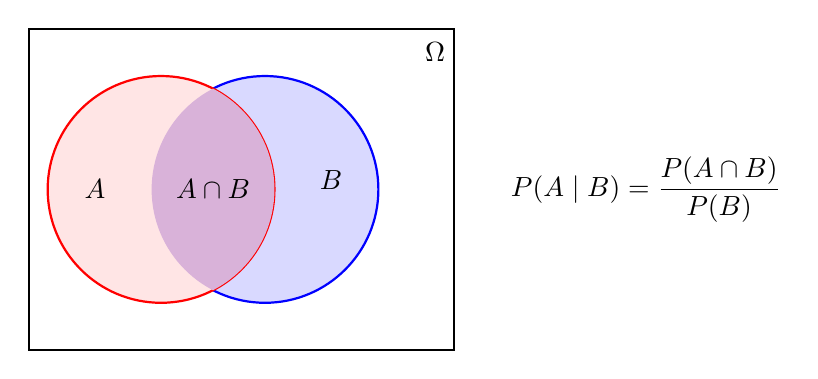
\begin{tikzpicture}[scale=1.2]

    % Sample space boundary
    \draw[thick] (-2,-1.7) rectangle (2.5,1.7);
    \node at (2.3,1.45) {$\Omega$};

    % Event B (shifted right)
    \draw[fill=blue!15, draw=blue, thick] (0.5,0) circle (1.2);
    \node at (1.2,0.1) {$B$};

    % Event A (shifted left)
    \draw[fill=red!10, draw=red, thick] (-0.6,0) circle (1.2);
    \node at (-1.3,0) {$A$};

    % Smaller intersection A ∩ B
    \begin{scope}
        \clip (0.5,0) circle (1.2);
        \fill[red!50!blue!30] (-0.6,0) circle (1.2);
    \end{scope}

	\node at (-0.05,0) {$A\cap B$};

    % Formula outside the sample space, to the right
    \node[anchor=west] at (3.0, 0) {$P(A\mid B)=\dfrac{P(A\cap B)}{P(B)}$};

\end{tikzpicture}
\caption{Conditional Probability Visualized.}
\label{figdef}
\end{figure}



%%%%%%%%%%%%%%%%%%%%%%%%%%%%%%%%%%%%%%%%%%%%%%%%%%%%%%%%%%%%%%%%%%%%%%%%%%%%%%%%%%%%%%%%%%%%%%%%%%%%%%
\section*{Theoretical Tools:}
%%%%%%%%%%%%%%%%%%%%%%%%%%%%%%%%%%%%%%%%%%%%%%%%%%%%%%%%%%%%%%%%%%%%%%%%%%%%%%%%%%%%%%%%%%%%%%%%%%%%%%

\noindent \subsection*{Multiplication Rule}

The definition immediately yields the \textbf{multiplication rule}:
\[
P(A \cap B) = P(B) P(A \mid B) = P(A) P(B \mid A).
\]
This is fundamental for computing joint probabilities when conditional probabilities are known.

\subsection*{Law of Total Probability}

If $\{B_1, B_2, \ldots, B_n\}$ forms a partition of the sample space with $P(B_i) > 0$ for each $1\le i\le n$, then
\[
P(A) = \sum_{i=1}^n P(A \mid B_i)\,P(B_i).
\]
This is useful when the occurrence of $A$ depends on several underlying scenarios $B_i$. See Figure \ref{figlawtotprob}. It is our main tool when we apply a ``divide and conquer" strategy to probability calculations.
\vskip 5mm
Here is a classic example of  total probability related to disease testing. Suppose 5\% of a population has a certain disease and there is a diagnostic test for the disease with the following characteristics:
\[P(\text{Positive}\mid\text{Disease})=0.95\quad P(\text{Negative}\mid\text{No Disease})=0.90.\]
Let $D$ be the event that a randomly selected person has the disease, and $D^c$ its complement. Let $T^+$ denote the event that the test is positive.  We can compute the probability that a randomly selected person's test is positive using the Law of Total Probability:
\[P(T^+)=P(T^+\cap D)+P(T^+\cap D^c)=P(T^+\mid D)P(D)+P(T^+\mid D^c)P(D^c).\]
Substitute the numbers:
\[P(T^+)=(0.95)(0.05)+(1-0.90)(0.95)=0.0475+0.095=0.1425.\]
Therefore, the probability that a randomly selected person's test is positive is $0.1425$.
\vskip 5mm
\begin{figure}[h!]
\centering
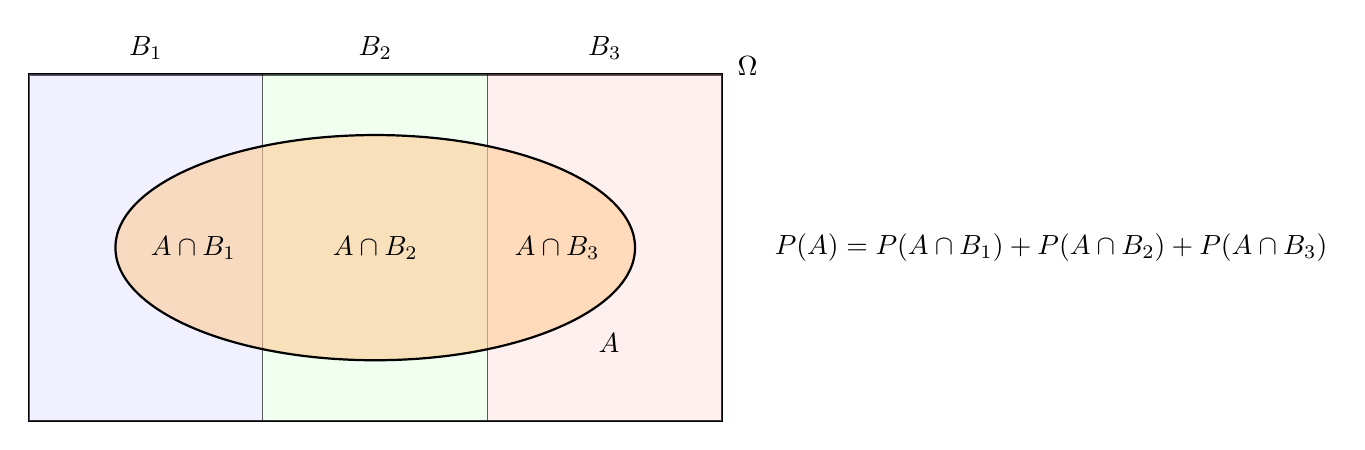
\begin{tikzpicture}[scale=1.1]

% Sample space
\draw[thick] (0,0) rectangle (8,4);
\node at (8.3,4.1) {$\Omega$};

% Partition blocks B1, B2, B3
\draw[fill=blue!15, opacity=0.4] (0,0) rectangle (2.7,4);
\node at (1.35,4.3) {$B_1$};

\draw[fill=green!15, opacity=0.4] (2.7,0) rectangle (5.3,4);
\node at (4,4.3) {$B_2$};

\draw[fill=red!15, opacity=0.4] (5.3,0) rectangle (8,4);
\node at (6.65,4.3) {$B_3$};

% Event A as an ellipse with visible black boundary
\begin{scope}
\clip (0,0) rectangle (8,4);
\fill[orange!40, opacity=0.6] (4,2) ellipse (3cm and 1.3cm);
\draw[thick, black] (4,2) ellipse (3cm and 1.3cm);
\end{scope}
\node at (6.7,0.9) {$A$};

% Labels for intersections A ∩ B_i
\node at (1.9,2) {$A \cap B_1$};
\node at (4,2) {$A \cap B_2$};
\node at (6.1,2) {$A \cap B_3$};

% Formula to the right of the figure
\node[right] at (8.5,2) {
$P(A)=P(A\cap B_1)+P(A\cap B_2)+P(A\cap B_3)$
};

\end{tikzpicture}
\caption{Law of Total Probability Illustrated.}
\label{figlawtotprob}
\end{figure}

\subsection*{Bayes' Rule}

An immediate consequence of the multiplication rule is the famous \textbf{Bayes' Rule}:
\[
P(B \mid A)
= \frac{P(A \mid B)\,P(B)}{P(A)}
= \frac{P(A \mid B)\,P(B)}{\sum_{i=1}^n P(A \mid B_i)\,P(B_i)}.
\]

Bayes' Rule allows inversion of conditional probabilities (from $P(A \mid B)$ to $P(B \mid A)$)
and is essential in Bayesian statistics, medical testing, reliability theory, and machine learning. 
We will visit Bayes' Rule in more detail in the following sections.

\subsection*{Geometric Interpretation}

When $A$ and $B$ are subsets of a finite or geometric sample space, $P(A\mid B)$ can be visualized as:
\[P(A\mid B) = \frac{\text{Area}(A \cap B)}{\text{Area}(B)}.\]
This is particularly useful for:
\begin{itemize}
    \item uniform distributions on geometric regions,
    \item problems involving continuous densities,
    \item visual intuition for event restriction.
\end{itemize}

\subsection*{Independence}

Events $A$ and $B$ are said to be \textbf{independent} if
\[P(A \cap B)=P(A)P(B).\]
or equivalently,
\[P(A\mid B)=P(A),\]
This formalizes the idea that knowledge of $B$ does not affect the probability of $A$.

\subsection*{Interpretation Through Simulation}

In practice, conditional probabilities can be approximated via Monte Carlo simulation:
\[
\widehat{P}_n(A \mid B)
= \frac{\#\{A \cap B \text{ occurs}\}}{\#\{B \text{ occurs}\}}.
\]
By the Law of Large Numbers (coming in the future), this empirical estimate converges to $P(A\mid B)$ as $n\to\infty$.
This provides a practical numerical approach when analytical computation is difficult.

\subsection*{Summary}

Conditional probability allows us to:
\begin{itemize}
    \item update probabilities when information becomes available,
    \item compute joint probabilities via the multiplication rule,
    \item express complex probability structures through the law of total probability,
    \item invert conditional relationships using Bayes' Rule,
    \item perform reasoning necessary for Bayesian inference and statistical learning.
\end{itemize}

It forms one of the central pillars of probability theory and is essential for understanding real-world uncertainty.



%%%%%%%%%%%%%%%%%%%%%%%%%%%%%%%%%%%%%
\section*{Example Problems}
%%%%%%%%%%%%%%%%%%%%%%%%%%%%%%%%%%%%


\begin{enumerate}

\item Let $A$ and $B$ be events with $P(A)=0.4$, $P(B)=0.5$, and $P(A\cap B)=0.2$.
    \begin{enumerate}
        \item Compute $P(A\mid B)$.
        \item Compute $P(B\mid A)$.
    \end{enumerate}

\item A box contains 6 good and 4 defective items. Two are drawn at random without replacement.
    \begin{enumerate}
        \item Find $P(\text{2nd is good} \mid \text{1st is good})$.
        \item Verify your result with a simulation.
    \end{enumerate}

\item A random variable $X \sim \text{Uniform}(0,1)$. Compute:
\[
P(X > 0.8 \mid X > 0.2).
\]

\item A six-sided die is rolled twice. Let  
    \[
    A = \{\text{sum is 8}\},\quad B = \{\text{first roll is 4}\}.
    \]
    Compute $P(A\mid B)$.

\end{enumerate}

\vskip 1cm

%==============================================
\paragraph*{Solutions}
%==============================================

\begin{enumerate}

\item
    \begin{align*}
    P(A\mid B) &= \frac{P(A\cap B)}{P(B)} = \frac{0.2}{0.5} = 0.4, \\
    P(B\mid A) &= \frac{P(A\cap B)}{P(A)} = \frac{0.2}{0.4} = 0.5.
    \end{align*}

\item  
\begin{enumerate}
    \item First item good: 6 good out of 10.  
    Remaining: 5 good out of 9.  
    \[
    P(\text{2nd good} \mid \text{1st good}) = \frac{5}{9}.
    \]

    \item Simulation matches $\approx 0.555\,.$
\end{enumerate}

\item
\[
P(X>0.8 \mid X>0.2) = \frac{0.2}{0.8} = 0.25.
\]

\item  
Given first roll is 4, the second roll must be 4 to make 8.  
\[
P(A\mid B) = P(\text{second roll is 4}) = \frac{1}{6}.
\]

\end{enumerate}



%%%%%%%%%%%%%%%%%%%%%%%%%%%%%%%%%%%%%%%%%%%%%%%%%%%%%%%%%%%%%%%%%%%%%%%%%%%%%%%%%%%%%%%%%%%%%%%%%%%%%%
\section*{Simulations:}
%%%%%%%%%%%%%%%%%%%%%%%%%%%%%%%%%%%%%%%%%%%%%%%%%%%%%%%%%%%%%%%%%%%%%%%%%%%%%%%%%%%%%%%%%%%%%%%%%%%%%%




%%%%%%%%%%%%%%%%%%%%%%%%%%%%%%%%%%%%%%%%%%%%%%%%%%%%%%%%%%
\paragraph{Example \#1: Conditional Probability in an Urn:}
%%%%%%%%%%%%%%%%%%%%%%%%%%%%%%%%%%%%%%%%%%%%%%%%%%%%%%%%%%

Consider an urn containing 5 red balls and 3 blue balls. Two balls are drawn sequentially without replacement. Let us define the following events:

\[
R_1 = \text{first ball drawn is red}, \quad
R_2 = \text{second ball drawn is red}.
\]

We are interested in computing the conditional probability:

\[
P(R_2 \mid R_1) = \frac{P(R_1 \cap R_2)}{P(R_1)}.
\]

\subparagraph{Theoretical Solution:}

\begin{itemize}
    \item Total balls: 8 (5 red, 3 blue)
    \item Probability first ball is red:
    \[
    P(R_1) = \frac{5}{8}.
    \]
    \item Probability both first and second balls are red:
    \[
    P(R_1 \cap R_2) = \frac{5}{8} \cdot \frac{4}{7} = \frac{20}{56} = \frac{5}{14}.
    \]
    \item Conditional probability:
    \[
    P(R_2 \mid R_1) = \frac{P(R_1 \cap R_2)}{P(R_1)} = \frac{5/14}{5/8} = \frac{4}{7} \approx 0.571.
    \]
\end{itemize}

\subparagraph{Simulation Approach (R):}

We can verify this using a Monte Carlo simulation in \texttt{R}:

% Can also use verbatim environment
\begin{lstlisting}[language=R]
n_sims <- 20000
first_red <- logical(n_sims)
both_red  <- logical(n_sims)

for (i in seq_len(n_sims)) {
  urn <- c(rep("R", 5), rep("B", 3))
  draw <- sample(urn, 2, replace = FALSE)
  first_red[i] <- (draw[1] == "R")
  both_red[i]  <- (draw[1] == "R" && draw[2] == "R")
}

p_first_red <- mean(first_red)
p_both_red  <- mean(both_red)
p_cond_emp  <- p_both_red / p_first_red
p_cond_theor <- 4/7
\end{lstlisting}

\subparagraph{Empirical Results:}

\begin{itemize}
    \item $P(\text{first red}) \approx$ empirical mean of \texttt{first\_red}
    \item $P(\text{both red}) \approx$ empirical mean of \texttt{both\_red}
    \item Empirical conditional probability:
    \[
    P(R_2 \mid R_1)_{\text{empirical}} \approx 0.571
    \]
    which converges to the theoretical value $4/7$ as the number of simulations increases.
\end{itemize}

\subparagraph{Visualizing Convergence:}

The running estimate of the conditional probability across simulations can be plotted (See Figure \ref{figcondproburn}):

% Can also use verbatim environment
\begin{lstlisting}[language=R]

set.seed(123) # (Optional) For Reproducibility
library(ggplot2)

n_sims <- 20000
first_red <- logical(n_sims)
both_red  <- logical(n_sims)

for (i in seq_len(n_sims)) {
  urn <- c(rep("R", 5), rep("B", 3))
  draw <- sample(urn, 2, replace = FALSE)
  first_red[i] <- (draw[1] == "R")
  both_red[i]  <- (draw[1] == "R" && draw[2] == "R")
}

p_first_red <- mean(first_red)
p_both_red  <- mean(both_red)
p_cond_emp   <- if (p_first_red > 0) p_both_red / p_first_red else NA_real_
p_cond_theor <- 4/7  # theoretical

cat("Urn results (n =", n_sims, ")\n")
print(data.frame(
  Quantity = c("P(first red)", "P(both red)", "P(2nd red | 1st red) empirical", 
  "Theoretical"),
  Value = c(p_first_red, p_both_red, p_cond_emp, p_cond_theor)
))

# running estimate
running <- data.frame(
  sim = seq_len(n_sims),
  cum_first = cumsum(first_red),
  cum_both  = cumsum(both_red)
)
running$cum_cond <- running$cum_both / running$cum_first

# Plot with FIX 1 (ignore NA rows, no warnings)
ggplot(running, aes(x = sim, y = cum_cond)) +
  geom_line(na.rm = TRUE) +   
  geom_hline(yintercept = p_cond_theor, linetype = "dashed") +
  labs(title = "Urn: convergence of P(2nd red | 1st red)",
       subtitle = "Urn with 5 red, 3 blue (draws without replacement)",
       x = "Simulations",
       y = "Estimated conditional probability") +
  theme_minimal()

\end{lstlisting}

\begin{figure}[h!]
\begin{center}
\includegraphics[scale=0.5]{cond_prob_simulation_urn}
\caption{Simulation of Conditional Probability Illustrated.}
\label{figcondproburn}
\end{center}
\end{figure}

The plot demonstrates that as the number of simulations increases, the empirical estimate of $P(R_2 \mid R_1)$ converges to the theoretical value $4/7$.
\vskip 1cm

%%%%%%%%%%%%%%%%%%%%%%%%%%%%%%%%%%%%%%%%%%%%%%%%%%%%%%%%%%
\paragraph{Example \#2: Conditional Probability with Dice Tokens:}
%%%%%%%%%%%%%%%%%%%%%%%%%%%%%%%%%%%%%%%%%%%%%%%%%%%%%%%%%%


Consider a bag containing the numbers $1,2,3,4,5,6$. Two numbers are drawn sequentially without replacement. Let us define the events:

\[E_1 = \text{first number drawn is even}, \quad
E_2 = \text{second number drawn is even}.\]

We want to compute the conditional probability:

\[P(E_2 \mid E_1) = \frac{P(E_1 \cap E_2)}{P(E_1)}.\]

\subparagraph{Theoretical Solution:}

\begin{itemize}
    \item There are 3 even numbers: $2,4,6$; and 3 odd numbers: $1,3,5$.
    \item Probability first number is even:
\[P(E_1) = \frac{3}{6} = \frac{1}{2}.\]
    \item Probability both first and second numbers are even:
\[P(E_1 \cap E_2) = \frac{3}{6} \cdot \frac{2}{5} = \frac{6}{30} = \frac{1}{5}.\]
    \item Conditional probability:
\[P(E_2 \mid E_1) = \frac{P(E_1 \cap E_2)}{P(E_1)} = \frac{1/5}{1/2} = \frac{2}{5} = 0.4.\]
\end{itemize}

\subparagraph{Simulation Approach (R):}

We can verify this using a Monte Carlo simulation:

% Can also use verbatim environment
\begin{lstlisting}[language=R]  

n_sims <- 20000
first_even  <- logical(n_sims)
second_even <- logical(n_sims)

for (i in seq_len(n_sims)) {
  bag <- 1:6
  draw <- sample(bag, 2, replace = FALSE)
  first_even[i]  <- (draw[1] %% 2 == 0)
  second_even[i] <- (draw[2] %% 2 == 0)
}

p_first_even <- mean(first_even)
p_both_even  <- mean(first_even & second_even)
p_cond_emp   <- p_both_even / p_first_even
p_cond_theor <- 2/5

\end{lstlisting}

\subparagraph{Empirical Results:}

\begin{itemize}
    \item $P(\text{first even}) \approx$ empirical mean of \texttt{first\_even}
    \item $P(\text{both even}) \approx$ empirical mean of \texttt{first\_even \& second\_even}
    \item Empirical conditional probability:
    \[
    P(E_2 \mid E_1)_{\text{empirical}} \approx 0.4
    \]
    which converges to the theoretical value $2/5$ as the number of simulations increases.
\end{itemize}

\subparagraph{Visualizing Convergence:}

The running estimate of $P(E_2 \mid E_1)$ across simulations can be plotted (See Figure \ref{figcondprobdie}):

% Can also use verbatim environment
\begin{lstlisting}[language=R]

## Dice tokens 1..6 drawn without replacement - P(2nd even | 1st even)
set.seed(456) # (Optional) For Reproducibility

library(ggplot2)

n_sims <- 20000
first_even  <- logical(n_sims)
second_even <- logical(n_sims)

for (i in seq_len(n_sims)) {
  bag <- 1:6
  draw <- sample(bag, 2, replace = FALSE)
  first_even[i]  <- (draw[1] %% 2 == 0)
  second_even[i] <- (draw[2] %% 2 == 0)
}

p_first_even <- mean(first_even)
p_both_even  <- mean(first_even & second_even)
p_cond_emp   <- if (p_first_even > 0) 
	p_both_even / p_first_even else NA_real_
p_cond_theor <- 2/5   # theoretical = 0.4

cat("Dice tokens results (n =", n_sims, ")\n")
print(data.frame(
  Quantity = c("P(first even)", "P(both even)", "P(2nd even | 1st even) 
  empirical", "Theoretical"),
  Value = c(p_first_even, p_both_even, p_cond_emp, p_cond_theor)
))

# Running estimate
running <- data.frame(
  sim       = seq_len(n_sims),
  cum_first = cumsum(first_even),
  cum_both  = cumsum(first_even & second_even)
)
running$cum_cond <- running$cum_both / running$cum_first

# Plot with FIX 1 (ignore NA rows)
ggplot(running, aes(x = sim, y = cum_cond)) +
  geom_line(na.rm = TRUE) +    # <-- FIX APPLIED
  geom_hline(yintercept = p_cond_theor, linetype = "dashed") +
  labs(
    title = "Dice Tokens: Convergence of P(2nd Even | 1st Even)",
    subtitle = "Draw without replacement from {1,2,3,4,5,6}",
    x = "Simulations",
    y = "Estimated conditional probability"
  ) +
  theme_minimal()
  
\end{lstlisting}

\begin{figure}[h!]
\begin{center}
\includegraphics[scale=0.5]{cond_prob_simulation_die}
\caption{Simulation of Conditional Probability Illustrated.}
\label{figcondprobdie}
\end{center}
\end{figure}


The plot demonstrates that as the number of simulations increases, the empirical estimate converges to the theoretical value $2/5 = 0.4$.


%%%%%%%%%%%%%%%%%%%%%%%%%%%%%%%%%%%%%%%%%%%%%%%%%%%%%%%%%%%%%%%%%%%%%%%%%%%%%%%%
\paragraph{Example \#3: Conditional Probability with Uniform(0,1) Variables}
%%%%%%%%%%%%%%%%%%%%%%%%%%%%%%%%%%%%%%%%%%%%%%%%%%%%%%%%%%%%%%%%%%%%%%%%%%%%%%%%


Here is an example related to drawing two numbers at random from the continuous interval $[0,1]$. Consider two independent random variables $X$ and $Y$, each uniformly distributed on $[0,1]$. We are interested in the events:
\[B = \{ X > 0.5 \},\quad A = \{ X + Y > 1 \}.\]
We want to compute the **conditional probability**:
\[P(A \mid B)=\frac{P(A \cap B)}{P(B)}.\]

\subparagraph{Theoretical Solution:}

\begin{itemize}
    \item Probability $B$ occurs:
\[P(B) = P(X > 0.5) = 0.5.\]
    \item Probability $A \cap B$ occurs: Since $X$ and $Y$ are independent and uniformly distributed, for $X>0.5$ the condition $X+Y>1$ is equivalent to $Y > 1-X$. Thus:
\[P(A \cap B) = \int_{0.5}^{1} P(Y > 1-x) \, dx = \int_{0.5}^{1} (1 - (1-x)) \, dx = \int_{0.5}^{1} x \, dx = \frac{3}{8}.\]
    \item Conditional probability:
\[P(A \mid B) = \frac{P(A \cap B)}{P(B)} = \frac{3/8}{1/2} = \frac{3}{4} = 0.75.\]
\end{itemize}

\subparagraph{Simulation Approach (R):}

We can verify this using a Monte Carlo simulation:

% Can also use verbatim environment
\begin{lstlisting}[language=R]  
n_sims <- 20000
X <- runif(n_sims)
Y <- runif(n_sims)

B <- (X > 0.5)
A <- (X + Y > 1)

p_B         <- mean(B)
p_A_and_B   <- mean(A & B)
p_cond_emp  <- p_A_and_B / p_B
p_cond_theor <- 3/4
\end{lstlisting}


\subparagraph{Empirical Results:}

\begin{itemize}
    \item $P(X>0.5) \approx$ empirical mean of \texttt{B}
    \item $P(X+Y>1 \text{ and } X>0.5) \approx$ empirical mean of \texttt{A \& B}
    \item Empirical conditional probability:
    \[
    P(A \mid B)_{\text{empirical}} \approx 0.75
    \]
    which converges to the theoretical value $3/4$ as the number of simulations increases.
\end{itemize}

\subparagraph{Visualizing Convergence:}

We can plot the running estimate of the conditional probability (See Figure \ref{figcondprobuni}):


% Can also use verbatim environment
\begin{lstlisting}[language=R]  

## Uniform(0,1) pair - P(X+Y > 1 | X > 0.5)

set.seed(789)
library(ggplot2)

n_sims <- 20000
X <- runif(n_sims)
Y <- runif(n_sims)

B <- (X > 0.5)
A <- (X + Y > 1)

p_B         <- mean(B)
p_A_and_B   <- mean(A & B)
p_cond_emp  <- if (p_B > 0) p_A_and_B / p_B else NA_real_
p_cond_theor <- 3/4   # theoretical = 0.75

cat("Uniform example results (n =", n_sims, ")\n")
print(data.frame(
  Quantity = c(
    "P(X>0.5)",
    "P(X+Y>1 and X>0.5)",
    "P(X+Y>1 | X>0.5) empirical",
    "Theoretical"
  ),
  Value = c(p_B, p_A_and_B, p_cond_emp, p_cond_theor)
))

# Running estimate
cum_B <- cumsum(B)
cum_A_and_B <- cumsum(A & B)
running <- data.frame(sim = seq_len(n_sims),
                      cum_cond = cum_A_and_B / cum_B)

# Plot with FIX 1 (ignore NA rows)
ggplot(running, aes(x = sim, y = cum_cond)) +
  geom_line(na.rm = TRUE) +   # <-- FIX APPLIED
  geom_hline(yintercept = p_cond_theor, linetype = "dashed") +
  labs(
    title = "Uniform(0,1): Convergence of P(X+Y>1 | X>0.5)",
    subtitle = "Theoretical value = 3/4",
    x = "Simulations",
    y = "Estimated conditional probability"
  ) +
  theme_minimal()

\end{lstlisting}


\begin{figure}[h!]
\begin{center}
\includegraphics[scale=0.5]{cond_prob_simulation_xyuni}
\caption{Simulation of Conditional Probability Illustrated.}
\label{figcondprobuni}
\end{center}
\end{figure}


The plot shows that as the number of simulations increases, the empirical estimate converges to the theoretical probability $3/4 = 0.75$.


%%%%%%%%%%%%%%%%%%%%%%%%%%%%%%%%%%%%%%%%%%%%%%%%%%%%%%%%%%%%%%%%%%%%%%%%%%%%%%%%%%%%%%%%%%%%%%%%%%%%%%%
%\section*{The R Code:} 
%%%%%%%%%%%%%%%%%%%%%%%%%%%%%%%%%%%%%%%%%%%%%%%%%%%%%%%%%%%%%%%%%%%%%%%%%%%%%%%%%%%%%%%%%%%%%%%%%%%%%%%
% Here is the R code used for the above simulations.
%\vspace*{2mm}
%\small 
%\begin{lstlisting}[language=R]
%
%
%\end{lstlisting}

\vskip 1cm
\hrule
\vskip 5mm
\begin{center}
\bf Please let me know if you have any questions, comments, or corrections!
\end{center}

%%%%%%%%%%%%%%%%%%%%%%%%%%%%%%%%%%%%%%%%%%%%%%%%%%%%%%
\end{document}
%%%%%%%%%%%%%%%%%%%%%%%%%%%%%%%%%%%%%%%%%%%%%%%%%%%%%%